\begin{frame}
    \frametitle{Particle Filter}
    \note{Information taken from Cyrill Stachniss's video https://youtu.be/MsYlueVDLI0}
    \footnotesize
    \begin{itemize}
        \item With EKF, we are restricted to Gaussian distributions.
        \item When we use EKF, we obtain a Gaussian distribution that describes where the robot is located.
        \item In Particle Filter, we use particles or hypotheses that describe where the robot could be.
        \item Instead of having a parametric form like EKF, which describes the probability distribution with the parameters mean $\mu$ and covariance $\covariance$, Partible Filter uses non-parametric samples as hypotheses about where the robot could be.
        
    \end{itemize}
    
    \begin{center}
        \movie[loop]{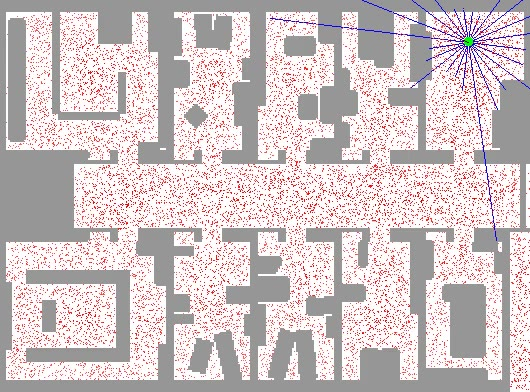
\includegraphics[width=0.4\columnwidth]{images/particle_filter/particle_filter_video.jpg}}{videos/particle_filter.mp4}
    \end{center}
    
    \note{Video taken from https://rse-lab.cs.washington.edu/projects/mcl/animations/global-floor.gif}
    
\end{frame}
    
\begin{frame}
    \frametitle{Flexible Function Approximation}
    \note{Information taken from Cyrill Stachniss's video https://youtu.be/MsYlueVDLI0}
    \footnotesize
    
    \begin{itemize}
        \item Goal: To be able to estimate any \textbf{arbitrary probability distribution}.
    \end{itemize}
    
    \begin{center}
        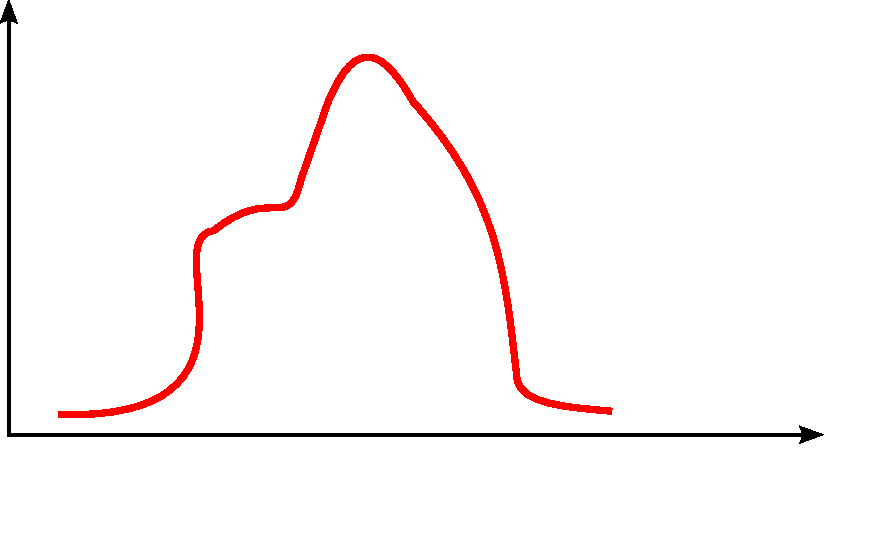
\includegraphics[width=0.5\columnwidth]{./images/particle_filter/arbitrary_distribution.pdf}
    \end{center}
    
\end{frame}
    
\begin{frame}
    \frametitle{Using Samples (Particles)}
    \note{Information taken from Cyrill Stachniss's video https://youtu.be/MsYlueVDLI0}
    \footnotesize
    \begin{itemize}
        \item \textbf{Multiple samples} to represent an arbitrary probability distribution
        \item Samples are more clustered in some areas and less so in others. The number of particles per unit area describes how likely it is that the robot is in that area.
        \item Each sample accumulates a bit of ``probability mass''
        \item Samples can be viewed as an approximation to the probability density function (pdf).
        \item To obtain the PDF, you must integrate over a certain area to obtain the mathematical probability that the robot is in that area.
    \end{itemize}
    
    \begin{center}
        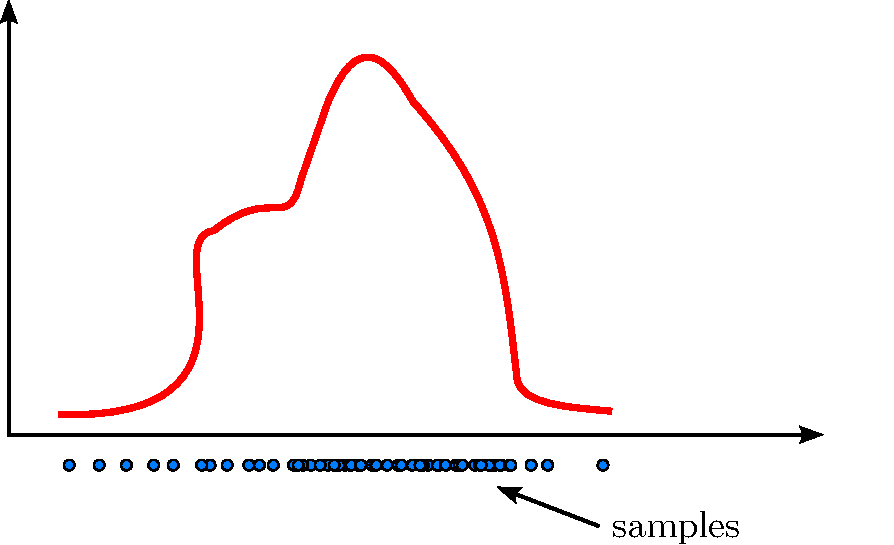
\includegraphics[width=0.5\columnwidth]{./images/particle_filter/arbitrary_distribution_samples.pdf}
    \end{center}
    
\end{frame}
    
\begin{frame}
    \frametitle{Using Weighted Samples}
    \note{Information taken from Cyrill Stachniss's video https://youtu.be/MsYlueVDLI0}
    \footnotesize
    \begin{itemize}
        \item \textbf{Multiple Weighted Samples} to Represent an Arbitrary Probability Distribution
        \item We can reduce the number of samples we need by adding weights to each sample.
        \item The more weight a sample has, the more probability mass there is in that region.
        \item The weights of all the particles together must sum to 1.
        \item Initially, we could add a uniform weight to each sample. For example, if we have $n$ samples, then each sample has weight $\frac{1}{n}$
    \end{itemize}

    \begin{center}
        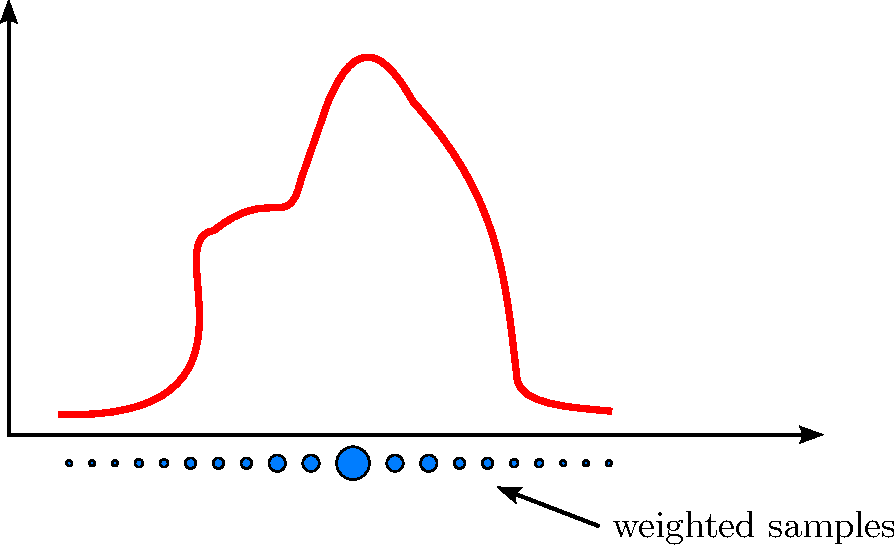
\includegraphics[width=0.5\columnwidth]{./images/particle_filter/arbitrary_distribution_weighted_samples.pdf}
    \end{center}

\end{frame}
    
\begin{frame}
    \frametitle{Particle Filter}
    \note{Information taken from Cyrill Stachniss's video https://youtu.be/MsYlueVDLI0}
    
    \footnotesize
    \begin{itemize}
        \item Note that this is an approximation of the PDF (\emph{Probabilistic Density Function}).
        \item It is important to have a sufficient number of samples to adequately represent the PDF.
    \end{itemize}

\end{frame}


\begin{frame}
    \frametitle{Particle Set}
    \note{Information extracted from Cyrill Stachniss' video https://youtu.be/MsYlueVDLI0}
    \begin{itemize}
        \item Set of weighted particles.
        \begin{center}
            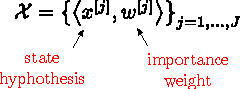
\includegraphics[width=0.5\columnwidth]{./images/particle_filter/weighted_samples.pdf}
        \end{center}
        \item The particles represent the posterior belief given by:
        \begin{equation*}
            p(x) = \sum_{j=1}^{J} w^{[j]} \delta_{x^{[j]}}(x),
        \end{equation*}
        where $\delta_{x^{[j]}}(x)$ is the Dirac delta function centered at the particle's location $x^{[j]}$.
        \begin{equation*}
            \delta(y) = 
            \begin{cases} 
            \infty, & y = x^{[j]} \\ 
            0, & y \neq x^{[j]} 
            \end{cases}.
        \end{equation*}
        \note{The function tends to infinity when $x = j$ and is equal to 0 for any other value of $x$.}
    \end{itemize}
\end{frame}

\begin{frame}
    \frametitle{Particles for Approximation}
    \note{Information extracted from Cyrill Stachniss' video https://youtu.be/MsYlueVDLI0}
    \begin{itemize}
        \item Particles to approximate a function.
        \begin{center}
            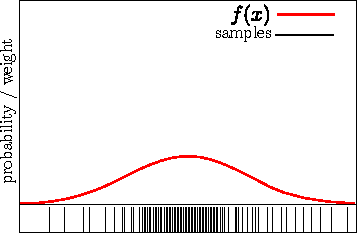
\includegraphics[width=0.45\columnwidth]{./images/particle_filter/gaussian_approximation_by_sampling.pdf}
            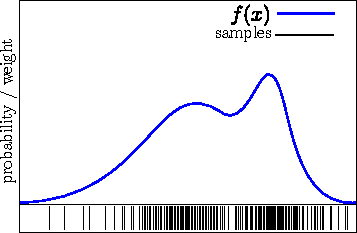
\includegraphics[width=0.45\columnwidth]{./images/particle_filter/particles_for_approximation.pdf}
        \end{center}
        \item The more particles in a region, the higher the probability of the region.
    \end{itemize}
    \begin{center}
        \alert{How to obtain such samples?}
    \end{center}
\end{frame}

\begin{frame}
    \frametitle{Closed-Form Sampling is Only Possible for Few Distributions}
    \note{Information extracted from Cyrill Stachniss' video https://youtu.be/MsYlueVDLI0}
    \begin{itemize}
        \item Example: Gaussian distribution.
        \begin{center}
            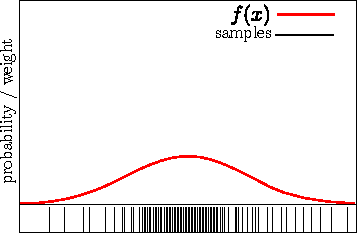
\includegraphics[width=0.5\columnwidth]{./images/particle_filter/gaussian_approximation_by_sampling.pdf}
        \end{center}
        \begin{equation*}
            x \leftarrow \frac{1}{2} \sum_{i=1}^{12} \text{rand}(-\sigma, \sigma)
        \end{equation*}
    \end{itemize}
    How to sample using another distribution?
    \note{Rejection sampling technique. Not used in particle filters because it is very inefficient.}
    \note{Importance Sampling Principle technique.}
\end{frame}

\begin{frame}
    \frametitle{Importance Sampling Principle}
    \note{Information extracted from Cyrill Stachniss' video https://youtu.be/MsYlueVDLI0}
    \begin{itemize}
        \item We can use a different distribution $\pi$ to generate samples from $f$.
        \item Consider the "differences between $\pi$ and $f$" using a weight $w = f(x) / \pi(x)$.
        \item Target: $f$.
        \item Proposal: $\pi$.
        \item Precondition: $f(x) > 0 \implies \pi(x) > 0$.
        \begin{center}
            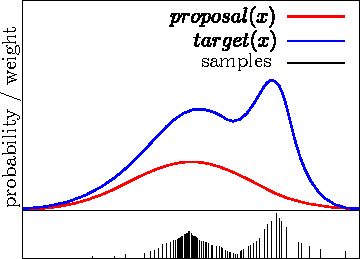
\includegraphics[width=0.45\textwidth]{./images/particle_filter/importance_sampling_principle.pdf}
        \end{center}
    \end{itemize}
\end{frame}

\begin{frame}
    \frametitle{Particle Filter}
    \note{Information extracted from Cyrill Stachniss' video https://youtu.be/MsYlueVDLI0}
    \begin{itemize}
        \item Recursive Bayesian filter.
        \item Non-parametric approach.
        \item Models the distribution using samples.
        \item \textbf{Prediction}: Sample from the proposal distribution.
        \item \textbf{Correction}: Weight by the ratio between the target and proposal distributions.
        \item \alert{The more samples we use, the better the estimate!}
    \end{itemize}
\end{frame}

\begin{frame}
    \frametitle{Particle Filter Algorithm}
    \note{Information extracted from Cyrill Stachniss' video https://youtu.be/MsYlueVDLI0}
    \begin{enumerate}
        \item Sample particles using the proposal distribution.
        \begin{equation*}
            x_t^{[j]} \sim \text{proposal}(x_t | \ldots)
        \end{equation*}
        \item Compute importance weights.
        \begin{equation*}
            w_t^{[j]} = \frac{\text{target}(x_t^{[j]})}{\text{proposal}(x_t^{[j]})}
        \end{equation*}
        \item Resampling: Select particle $i$ with probability $w_t^{[j]}$ and repeat $J$ times.
    \end{enumerate}
    \note{Replace unlikely samples with more likely ones.}
\end{frame}

\begin{frame}
    \frametitle{Particle Filter Algorithm}
    \note{Information extracted from Cyrill Stachniss' video https://youtu.be/MsYlueVDLI0}
    \begin{algorithmic}[1]
        \Procedure{ParticleFilter}{$\mathcal{X}_{t-1}, u_{t}, z_{t}$}
        \State $\bar{\mathcal{X}}_t = \mathcal{X}_t = \emptyset$
        \For{$j = 1$ to $J$}
            \State Sample $x_t^{[j]} \sim \pi(x_t)$
            \State $w_t^{[j]} = \dfrac{p(x_t^{[j]})}{\pi(x_{t}^{[j]})}$
            \State $\bar{\mathcal{X}}_t = \bar{\mathcal{X}}_t + \langle x_t^{[j]}, w_t^{[j]}\rangle$
        \EndFor
        \For{$j = 1$ to $M$}
            \State Draw $i$ with probability $\propto w_t^{[i]}$
            \State Add $x_t^{[i]}$ to $\mathcal{X}_t$
        \EndFor
        \State Return $\mathcal{X}_t$
        \EndProcedure
    \end{algorithmic}
\end{frame}

\begin{frame}
    \frametitle{Monte Carlo Localization}
    \note{Information extracted from Cyrill Stachniss' video https://youtu.be/MsYlueVDLI0}
    Monte Carlo Localization: Particle Filter for robot localization.
\end{frame}

\begin{frame}
    \frametitle{Monte Carlo Localization}
    \note{Information extracted from Cyrill Stachniss' video https://youtu.be/MsYlueVDLI0}
    \begin{itemize}
        \item Each particle is a hypothesis of the pose.
        \item Proposal is the motion model:
        \begin{equation*}
            x_t^{[j]} \sim p(x_t \, | \, x_{t-1}, u_t)
        \end{equation*}
        \item Correction via the observation model:
        \begin{equation*}
            w_t^{[j]} = \frac{\text{target}}{\text{proposal}} \propto p(z_t \, | \, x_t, m)
        \end{equation*}
    \end{itemize}
\end{frame}

\begin{frame}
    \frametitle{Particle Filter for Localization}
    \note{Information extracted from Cyrill Stachniss' video https://youtu.be/MsYlueVDLI0}
    \begin{algorithmic}[1]
        \Procedure{ParticleFilter}{$\mathcal{X}_{t-1}, u_{t}, z_{t}$}
        \State $\bar{\mathcal{X}}_t = \mathcal{X}_t = \emptyset$
        \For{$j = 1$ to $J$}
            \State Sample $x_t^{[j]} \sim p(x_t \, | \, u_t, x_{t-1}^{[j]})$
            \State $w_t^{[j]} = p(z_t \, | \, x_t^{[j]})$
            \State $\bar{\mathcal{X}}_t = \bar{\mathcal{X}}_t + \langle x_t^{[j]}, w_t^{[j]}\rangle$
        \EndFor
        \For{$i = 1$ to $J$}
            \State Draw $i \in 1,\ldots,J$ with probability $\propto w_t^{[i]}$
            \State Add $x_t^{[i]}$ to $\mathcal{X}_t$
        \EndFor
        \State Return $\mathcal{X}_t$
        \EndProcedure
    \end{algorithmic}
\end{frame}

\begin{frame}
    \frametitle{Monte Carlo Localization - Correction Step}
    \note{Information extracted from Cyrill Stachniss' video https://youtu.be/MsYlueVDLI0}
    \begin{center}
        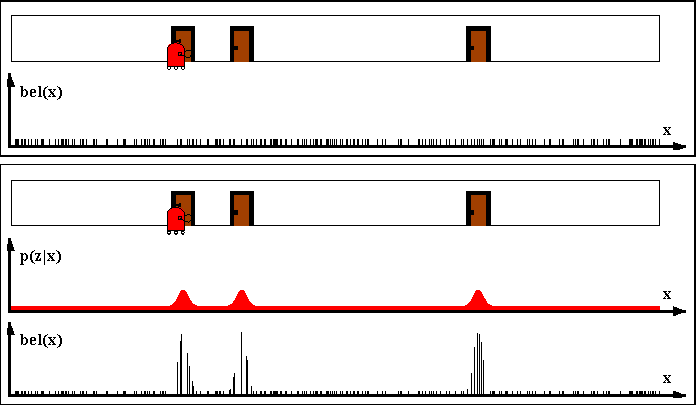
\includegraphics[width=0.8\textwidth]{./images/particle_filter/monte_carlo_correction.pdf}
    \end{center}
\end{frame}

\begin{frame}
    \frametitle{Monte Carlo Localization - Resampling and Prediction}
    \note{Information extracted from Cyrill Stachniss' video https://youtu.be/MsYlueVDLI0}
    \begin{center}
        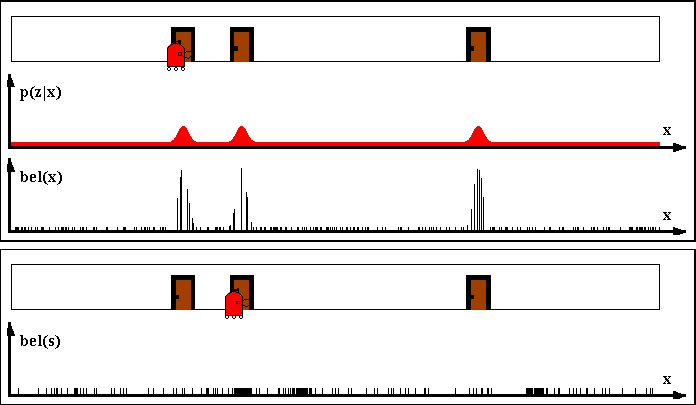
\includegraphics[width=0.8\textwidth]{./images/particle_filter/monte_carlo_resample_and_predict.pdf}
    \end{center}
\end{frame}

\begin{frame}
    \frametitle{Monte Carlo Localization - Correction Step 2}
    \note{Information extracted from Cyrill Stachniss' video https://youtu.be/MsYlueVDLI0}
    \begin{center}
        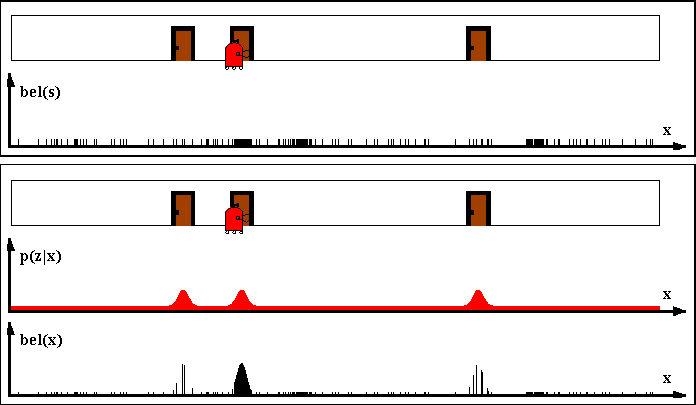
\includegraphics[width=0.8\textwidth]{./images/particle_filter/monte_carlo_correction2.pdf}
    \end{center}
\end{frame}

\begin{frame}
    \frametitle{Monte Carlo Localization - Resampling and Prediction 2}
    \note{Information extracted from Cyrill Stachniss' video https://youtu.be/MsYlueVDLI0}
    \begin{center}
        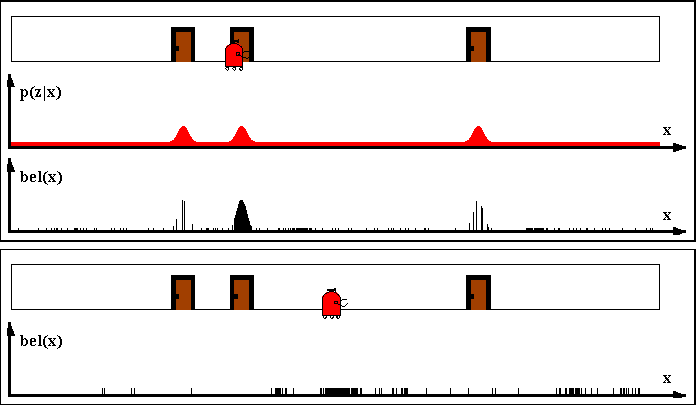
\includegraphics[width=0.8\textwidth]{./images/particle_filter/monte_carlo_resample_and_predict2.pdf}
    \end{center}
\end{frame}

\begin{frame}
    \frametitle{Resampling}
    \note{Information extracted from Cyrill Stachniss' video https://youtu.be/MsYlueVDLI0}
    \begin{itemize}
        \item Select particle $i$ with probability $w_t^{[i]}$. Repeat $J$ times.
        \item Informally: "Replace unlikely samples with more likely ones."
        \item Survival of the fittest.
        \item "Trick" to avoid many samples covering unlikely states.
        \item Necessary because we have a limited number of samples.
    \end{itemize}
\end{frame}

\begin{frame}
    \frametitle{Resampling Methods}
    \note{Information extracted from Cyrill Stachniss' video https://youtu.be/MsYlueVDLI0}
    \begin{overlayarea}{\textwidth}{\textheight}
        \only<1>{
            \begin{center}
                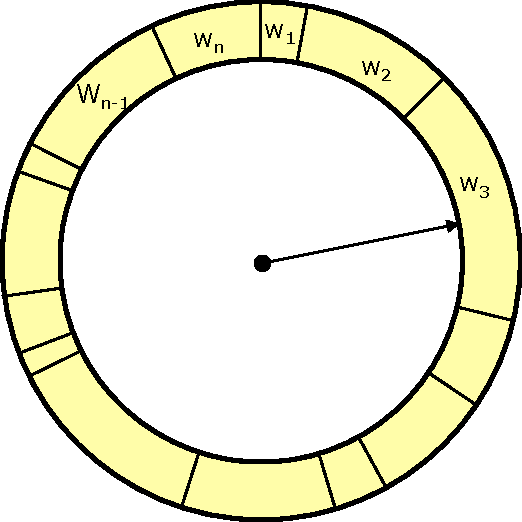
\includegraphics[width=0.35\textwidth]{./images/particle_filter/resampling_rulette_wheel1.pdf}
            \end{center}
        }
        \only<2>{
            \begin{center}
                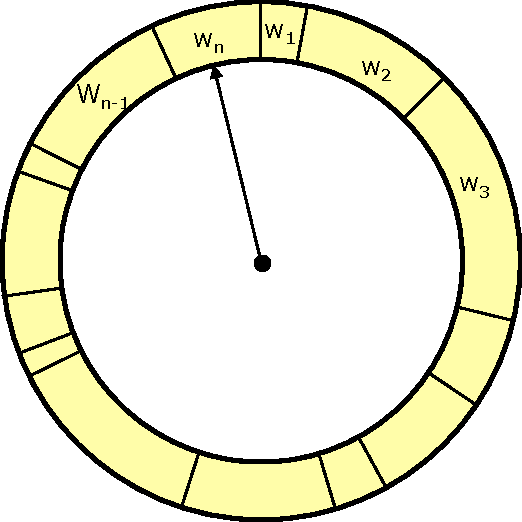
\includegraphics[width=0.35\textwidth]{./images/particle_filter/resampling_rulette_wheel2.pdf}
            \end{center}
        }
        \only<3>{
            \begin{center}
                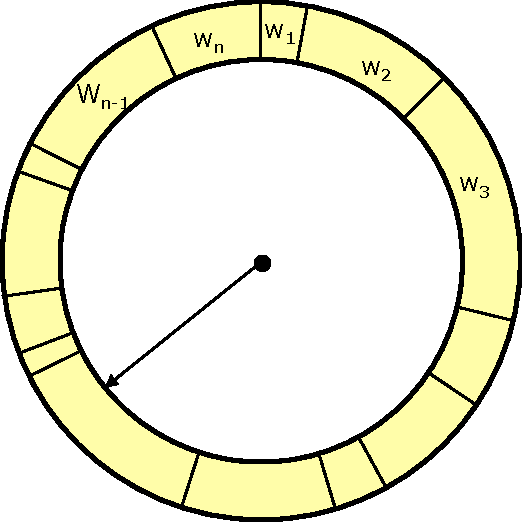
\includegraphics[width=0.35\textwidth]{./images/particle_filter/resampling_rulette_wheel3.pdf}
            \end{center}
        }
        \only<3>{
            \begin{itemize}
                \item Roulette Wheel.
                \item Binary search to determine which bucket the ball falls into ($O(J \log(J))$).
            \end{itemize}
            \note{The buckets on the roulette wheel represent the particles' weights. The larger the bucket, the more likely the particle is to be selected.}
            \note{We do this $J$ times. We determine where the ball lands using binary search. The sum of all weights on the wheel is 1. If we generate a random number between 0 and 1, we can use binary search to find the corresponding bucket.}
        }
    \end{overlayarea}
\end{frame}

\begin{frame}
    \frametitle{Resampling Methods}
    \note{Information extracted from Cyrill Stachniss' video https://youtu.be/MsYlueVDLI0}
    \begin{overlayarea}{\textwidth}{\textheight}
        \only<1>{
            \begin{center}
                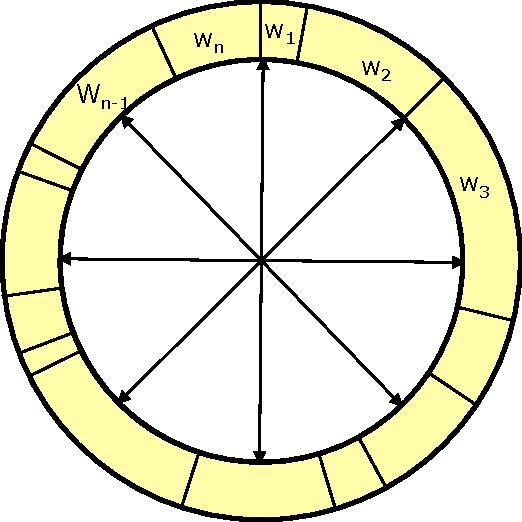
\includegraphics[width=0.35\textwidth]{./images/particle_filter/resampling_stochastic_universal_sampling1.pdf}
            \end{center}
        }
        \only<2>{
            \begin{center}
                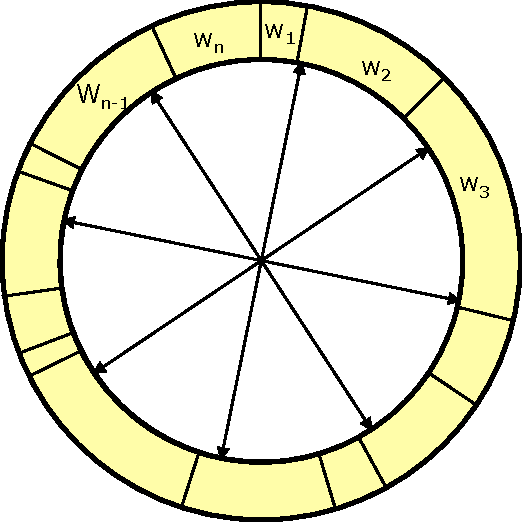
\includegraphics[width=0.35\textwidth]{./images/particle_filter/resampling_stochastic_universal_sampling2.pdf}
            \end{center}
        }
        \only<2>{
            \begin{itemize}
                \item Stochastic Universal Sampling (using $J$ equidistant arrows).
                \item Also called \emph{Low-Variance Resampling} (avoids rapid particle concentration).
                \item $O(J)$.
            \end{itemize}
            \note{Using arrows placed equidistantly. Rotate them together and select $n$ particles. Generate one random number and select all $J$ particles at once.}
            \note{Computational cost is linear because we only need to traverse the weights once to determine where all arrows land.}
            \note{Example: 8 arrows spaced 45 degrees apart.}
        }
    \end{overlayarea}
\end{frame}

\begin{frame}
    \frametitle{Resampling}
    \note{Information extracted from Cyrill Stachniss' video https://youtu.be/MsYlueVDLI0}
    \begin{itemize}
        \item Sampling with replacement (we sample a particle and then put it back in the bag).
        \item Roulette Wheel resampling is easy to understand but suboptimal in practice.
        \item \alert{What happens if all particles have the same weight?}
        \note{If all particles have the same weight, it's like having a sensor that provides no information.}
        \note{If all particles have the same weight, resampling will randomly select and duplicate some particles, while others will not be selected and will "die." This happens without any particle being better than another, leading the system to converge to an arbitrary location.}
        \note{Therefore, if all particles have the same weight, there is no reason to prefer one over another.}
    \end{itemize}
\end{frame}

\begin{frame}
    \frametitle{Low Variance Resampling Idea}
    \note{Information extracted from Cyrill Stachniss' video https://youtu.be/MsYlueVDLI0}
    \begin{center}
        \only<1>{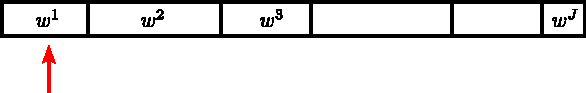
\includegraphics[width=0.7\textwidth]{./images/particle_filter/low_variance_resampling.pdf}}
        \only<2>{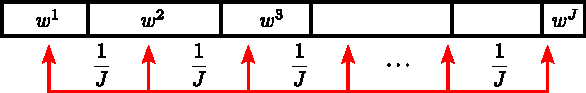
\includegraphics[width=0.7\textwidth]{./images/particle_filter/low_variance_resampling2.pdf}}
    \end{center}
    \begin{enumerate}
        \item<1-> Generate a random value $r$ between 0 and $\dfrac{1}{J}$.
        \item<2> Select $J-1$ particles in $\dfrac{1}{J}$ steps (based on cumulative weight).
    \end{enumerate}
\end{frame}

\begin{frame}
    \frametitle{Low Variance Resampling}
    \note{Information extracted from Cyrill Stachniss' video https://youtu.be/MsYlueVDLI0}
    \begin{center}
        \only<1>{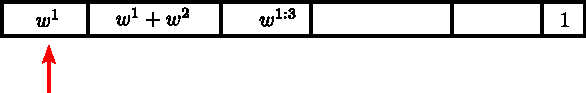
\includegraphics[width=0.7\textwidth]{./images/particle_filter/low_variance_resampling3.pdf}}
        \only<2>{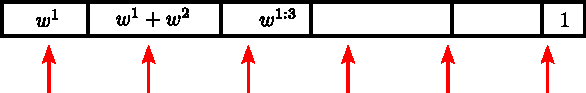
\includegraphics[width=0.7\textwidth]{./images/particle_filter/low_variance_resampling4.pdf}}
    \end{center}
    \begin{enumerate}
        \item<1-> Generate a random value $r$ between 0 and $\dfrac{1}{J}$.
        \item<2>
        \begin{algorithmic}[1]
            \For{$j = 1$ to $J$}
                \State $U = r + (j - 1) \dfrac{1}{J}$
                \While{$(U > \text{cum}[i])$}
                    \State $i++$
                \EndWhile
                \State Add $x_t^{[i]}$ to $\bar{\mathcal{X}}_t$
            \EndFor
        \end{algorithmic}
    \end{enumerate}
\end{frame}

\begin{frame}
    \frametitle{Low Variance Resampling}
    \begin{algorithmic}[1]
        \Procedure{LowVarianceResampling}{$\mathcal{X}_{t}$, $\mathcal{W}_{t}$}
        \State $\bar{\mathcal{X}}_t = \emptyset$
        \State $r = \text{rand}(0; J^{-1})$
        \State $c = w_t^{[1]}$
        \State $i = 1$
        \For{$j = 1$ to $J$}
            \State $U = r + (j - 1) J^{-1}$
            \While{$U > c$}
                \State $i = i + 1$
                \State $c = c + w_t^{[i]}$
            \EndWhile
            \State Add $x_t^{[i]}$ to $\bar{\mathcal{X}}_t$
        \EndFor
        \State Return $\bar{\mathcal{X}}_t$
        \EndProcedure
    \end{algorithmic}
\end{frame}

\begin{frame}
    \frametitle{Low Variance Resampling}
    \note{Information extracted from Cyrill Stachniss' video https://youtu.be/MsYlueVDLI0}
    \begin{itemize}
        \item Performs resampling that preserves samples when they have equal weights.
        \item Faster than Roulette Wheel resampling: $\mathcal{O}(J)$ vs. $\mathcal{O}(J \log J)$.
        \item \alert{We will always use Low Variance Resampling!}
    \end{itemize}
\end{frame}

\begin{frame}
    \frametitle{Disadvantages of Particle Filter}
    \note{Information extracted from Cyrill Stachniss' video https://youtu.be/MsYlueVDLI0}
    \begin{itemize}
        \item Does not scale well for high-dimensional spaces.
        \note{PF becomes computationally expensive because many particles are needed to cover the probability distribution. PF works well for low dimensions, up to 4, but beyond that, heuristics are needed to reduce the number of particles while keeping them representative.}
        \note{The number of particles grows exponentially with the state dimensions.}
        \item Problematic in situations with high uncertainty.
        \item \emph{Depletion Problem} (most particles have low weight).
        \note{The Depletion Problem: occurs when we have too few particles relative to the state dimensionality. The particles do not cover high-probability areas, causing them to "die" and the filter to eventually diverge.}
        \note{Example: Imagine 100 particles tracking a robot's position. If the robot makes a sharp turn, many particles will have low weights because they poorly predict the motion. After resampling, only a few particles "survive," and the filter loses diversity, affecting future estimates.}
    \end{itemize}
\end{frame}

\begin{frame}
    \frametitle{Advantages}
    \note{Information extracted from Cyrill Stachniss' video https://youtu.be/MsYlueVDLI0}
    \begin{itemize}
        \item Can work with non-Gaussian distributions.
        \item Works well in low-dimensional spaces.
        \item Can handle ambiguities in data association.
        \note{We can let each particle have its own way of associating data. Since there is no uncertainty associated with this, we can make decisions dependent on each particle and see which one survives.}
        \item Can easily incorporate different sensing modalities.
        \note{We can incorporate different sensing modalities by simply multiplying the weight with the computed weight from another sensor.}
        \item Robust.
        \note{Robust because even when models are imperfect, it can still compute good beliefs.}
        \item Easy to implement.
    \end{itemize}
\end{frame}

\begin{frame}
    \frametitle{Summary – Particle Filter}
    \note{Information extracted from Cyrill Stachniss' video https://youtu.be/MsYlueVDLI0}
    \begin{itemize}
        \item Particle filters are recursive, non-parametric Bayesian filters.
        \item The posterior belief is represented by a set of weighted samples.
        \item Not limited to Gaussian distributions.
        \item Proposal to draw samples at $t+1$.
        \item Weight to account for differences between the proposal and target.
        \item The art lies in designing suitable motion and sensing models.
    \end{itemize}
\end{frame}

\begin{frame}
    \frametitle{Summary – Localization with PF}
    \note{Information extracted from Cyrill Stachniss' video https://youtu.be/MsYlueVDLI0}
    \begin{itemize}
        \item Particles are propagated according to the motion model.
        \item Weighted by the observation probability.
        \item Called Monte Carlo Localization (MCL).
        \item MCL is the gold standard for mobile robot localization in \emph{indoor} environments.
    \end{itemize}
\end{frame}